\documentclass{beamer}
\usetheme{Darmstadt}
\usepackage{beamerthemesplit}
\usepackage{latexsym}
\usepackage{ae,aecompl}
\usepackage{graphicx}
\usepackage{amsfonts}
\usepackage{tikz}
\usepackage{graphics}
% \usepackage{url}

\graphicspath{{../images/}}

\hypersetup{
  pdftitle={The OpenDaylight Open Source Project},
  pdfauthor={Sergio Najib Arroutbi Braojos},
  pdfcreator={},
  pdfproducer=PDFLaTeX,
  pdfsubject={nn},
}

\title{The OpenDaylight Open Source Project}
\author{Sergio Najib Arroutbi Braojos}

\begin{document}

% Background Image
\setbeamertemplate{background}{%
    \tikz\node[opacity=0.1] at (current page.center) {
    \vbox to \paperheight{\vfil\hbox to \paperwidth{\hfil
\includegraphics[width=8cm]{opendaylight-logo-00.png}\hfil}\vfil}
 };

}

\frame{\titlepage
\begin{flushright}
{\tiny
(cc) 2014 Sergio Najib Arroutbi Braojos.
    This work is under a license Creative Commons CC-BY 3.0.\\
To view a copy of full license, see \url{http://creativecommons.org/licenses/by/3.0/}
}
\begin{figure}[h]
    \begin{flushright}
        
\includegraphics[width=0.6in]{by.png}
        \label{fig:by}
    \end{flushright}
\end{figure}
\end{flushright}
}

\section{About}

% Presentation
\begin{frame}[allowframebreaks]
\frametitle{About OpenDaylight}

\begin{itemize}
	\item FLOSS SDN Controller
 \item SDN/NFV: Next big Networking industry revolution
	\item Started in April 8, 2013
	\item Hosted by Linux Foundation
	\item Cisco, Ericsson, Juniper, IBM, HP, Microsoft, Red Hat, Dell, Citrix, Brocade
	\item Two releases: Hydrogen, Helium
\end{itemize}

\end{frame}

\section{About SDN}

\begin{frame}[allowframebreaks]
\frametitle{About SDN}

\begin{itemize}
 \item Separate Networking Control Logic from Networking Hardware
	\item Homogeneize Networking Resources Administration
 \item Opex Reduction
	\item Based on OpenFlow protocol
 \item SDN Architecture:\linebreak
	- Open Standards/Vendor-Neutral\linebreak
	- Directly Programmable\linebreak
	- Agile\linebreak
	- Centrally Managed\linebreak
	- Programmatically Configured
 \item OpenDaylight SDN Controller: Manage network devices through OpenFlow\linebreak
\end{itemize}

\end{frame}

\section{About SDN}

% Presentation
\begin{frame}[allowframebreaks]
\frametitle{About SDN}

\begin{center}
  \begin{figure}
    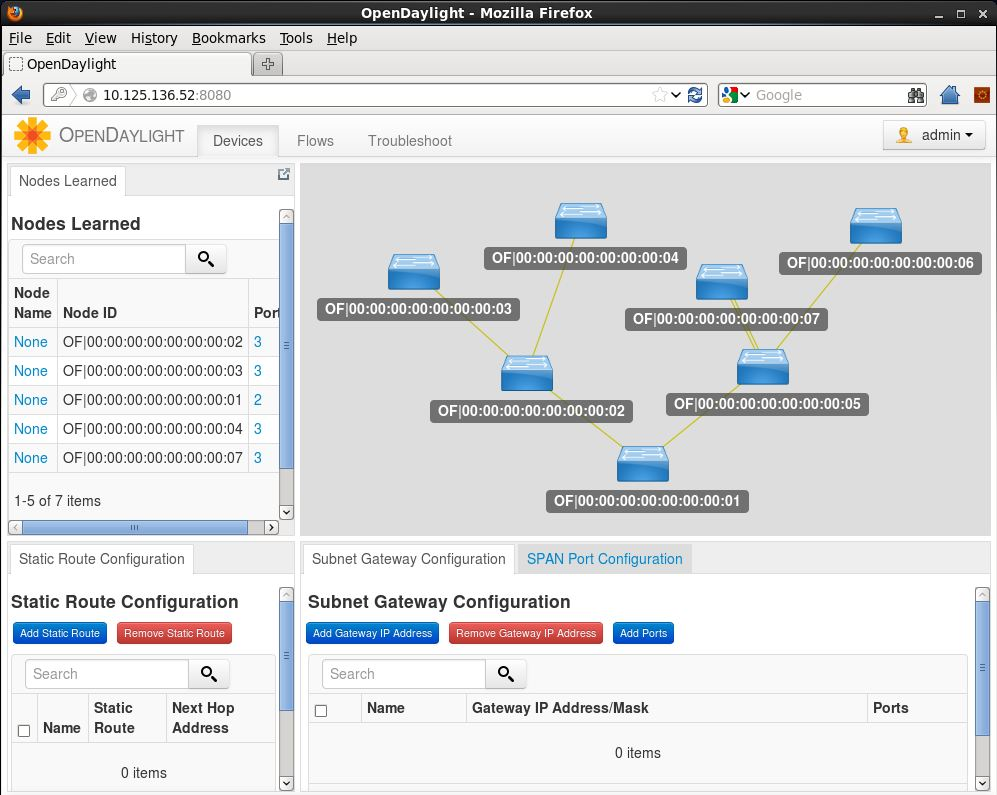
\includegraphics[width=8cm]{odl-controller-00.png}
  \end{figure}
\end{center}

\end{frame}

\section{About NFV}

% Presentation
\begin{frame}[allowframebreaks]
\frametitle{About NFV}

\begin{itemize}
 \item Network Virtualization (Network as Utility)
 \item Capex Reduction
 \item Hardware Homogeneization: Commodity Fragmentation to:\linebreak
	- Standard High Volume Servers\linebreak
	- Standard High Volume Storage\linebreak
	- Standard High Volume Ethernet Switches
\end{itemize}

\end{frame}

\section{About NFv}

% Presentation
\begin{frame}[allowframebreaks]
\frametitle{About NFV}

\begin{center}
  \begin{figure}
    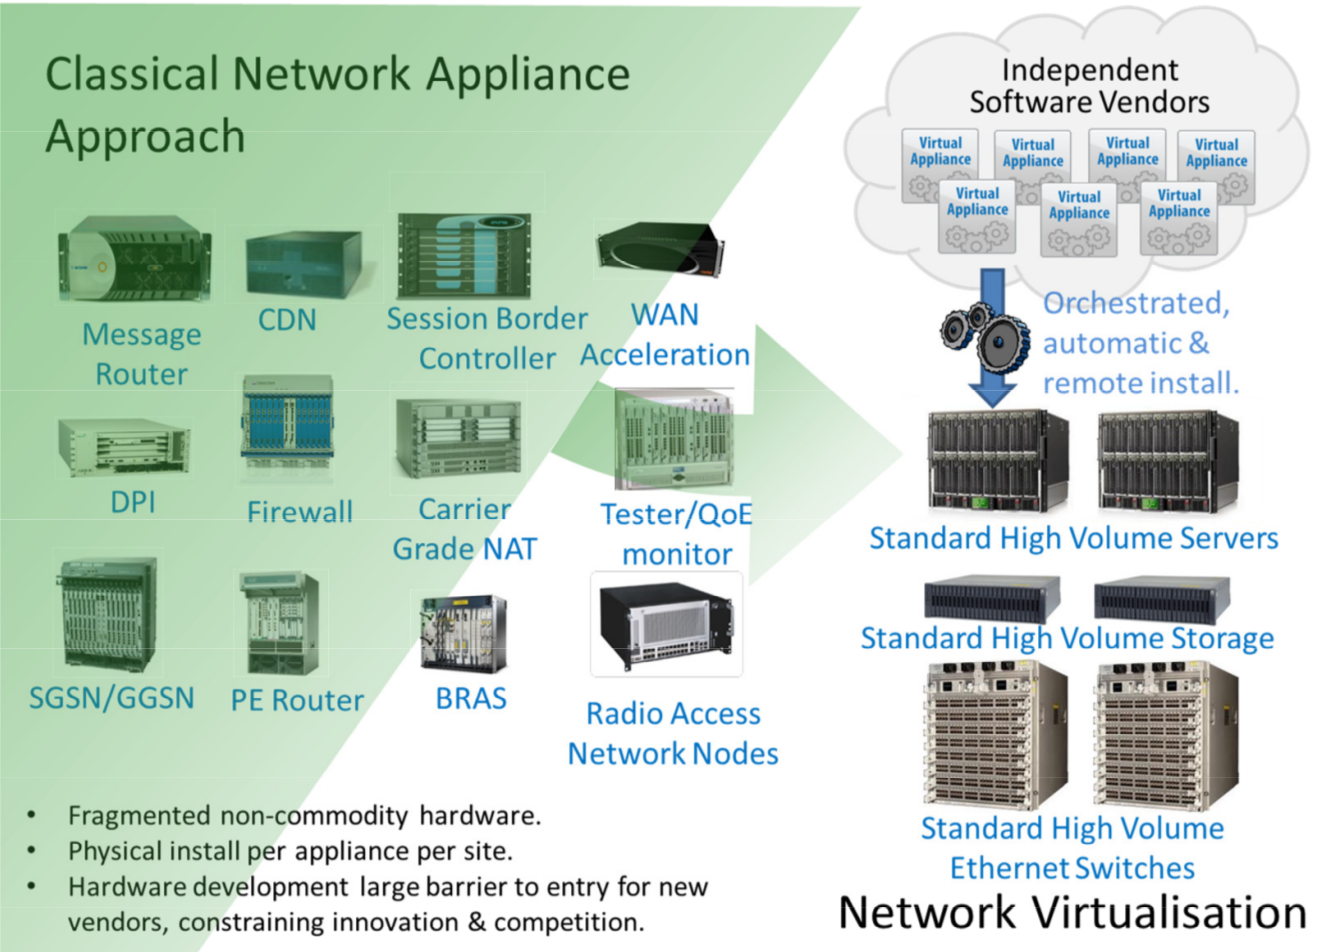
\includegraphics[width=9cm]{nfv-etsi-01.png}
  \end{figure}
\end{center}

\end{frame}

\section{SDN Market Estimations}

% Presentation
\begin{frame}[allowframebreaks]
\frametitle{SDN Market Estimations}

\begin{center}
  \begin{figure}
    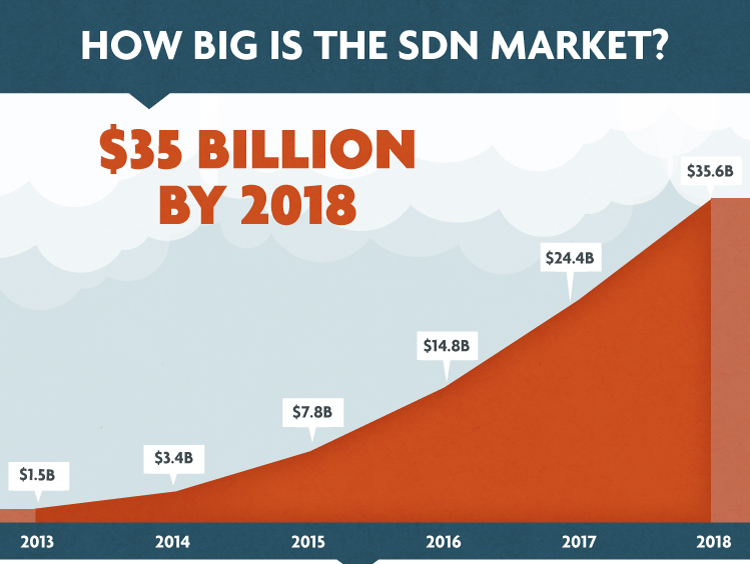
\includegraphics[width=9cm]{sdn-estimations-2018.png}
  \end{figure}
\end{center}

\end{frame}

\section{Economic Aspects}

% Presentation
\begin{frame}[allowframebreaks]
\frametitle{Economic Aspects}

\begin{itemize}
 \item Beginning of 2013:\linebreak
	- Big Expectations Market\linebreak
 - Big Impact on Networking Industry
 \item Late 2014:\linebreak
	- SDN/NFV: Open Technology, but complicated to implement\linebreak
	- Hardware Investment is needed\linebreak
	- Downward Corrections:
   \begin{itemize}
   \item Optimistics: \$8.0B by 2018
   \item Pesimistics: \$3.6B by 2019
   \end{itemize}
	- 2014: Hype Cycle: Towards Trough of Disillusionment
\end{itemize}

\end{frame}

\section{Economic Aspects}

% Presentation
\begin{frame}[allowframebreaks]
\frametitle{Economic Aspects}

\begin{center}
  \begin{figure}
    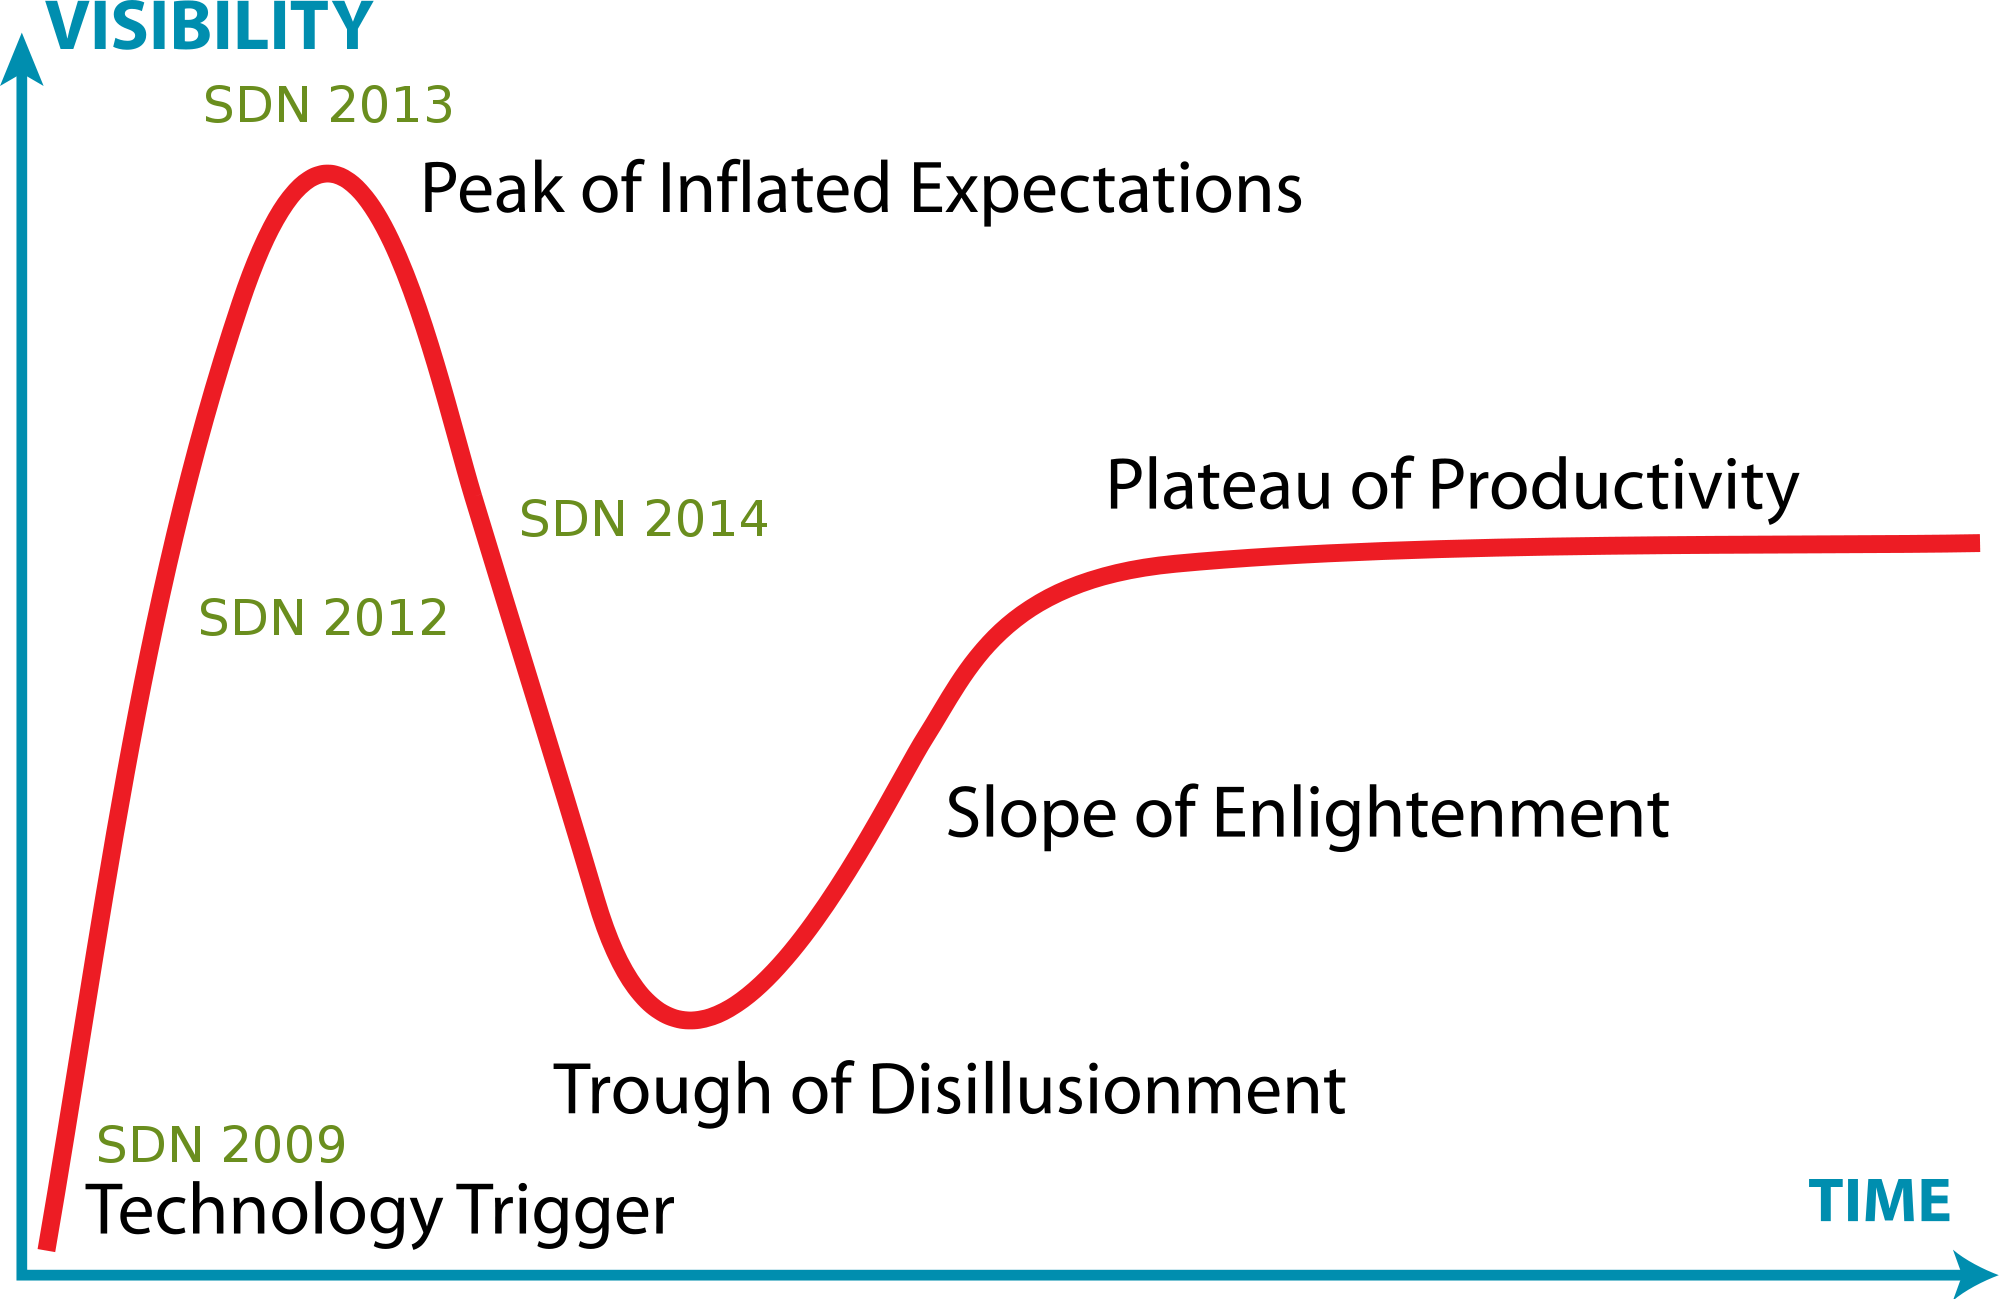
\includegraphics[width=9cm]{hype-cycle-03.png}
  \end{figure}
\end{center}

\end{frame}

\section{Economic Aspects}

% Presentation
\begin{frame}[allowframebreaks]
\frametitle{Economic Aspects}

\begin{center}
  \begin{figure}
    \includegraphics[width=9cm]{sdn-saves-capex.png}
  \end{figure}
\end{center}

\end{frame}

\section{Economic Aspects}

% Presentation
\begin{frame}[allowframebreaks]
\frametitle{Economic Aspects}

\begin{center}
  \begin{figure}
    \includegraphics[width=9cm]{sdn-saves-opex.png}
  \end{figure}
\end{center}

\end{frame}

\section{Economic Aspects}

% Presentation
\begin{frame}[allowframebreaks]
\frametitle{Economic Aspects}

\begin{center}
  \begin{figure}
    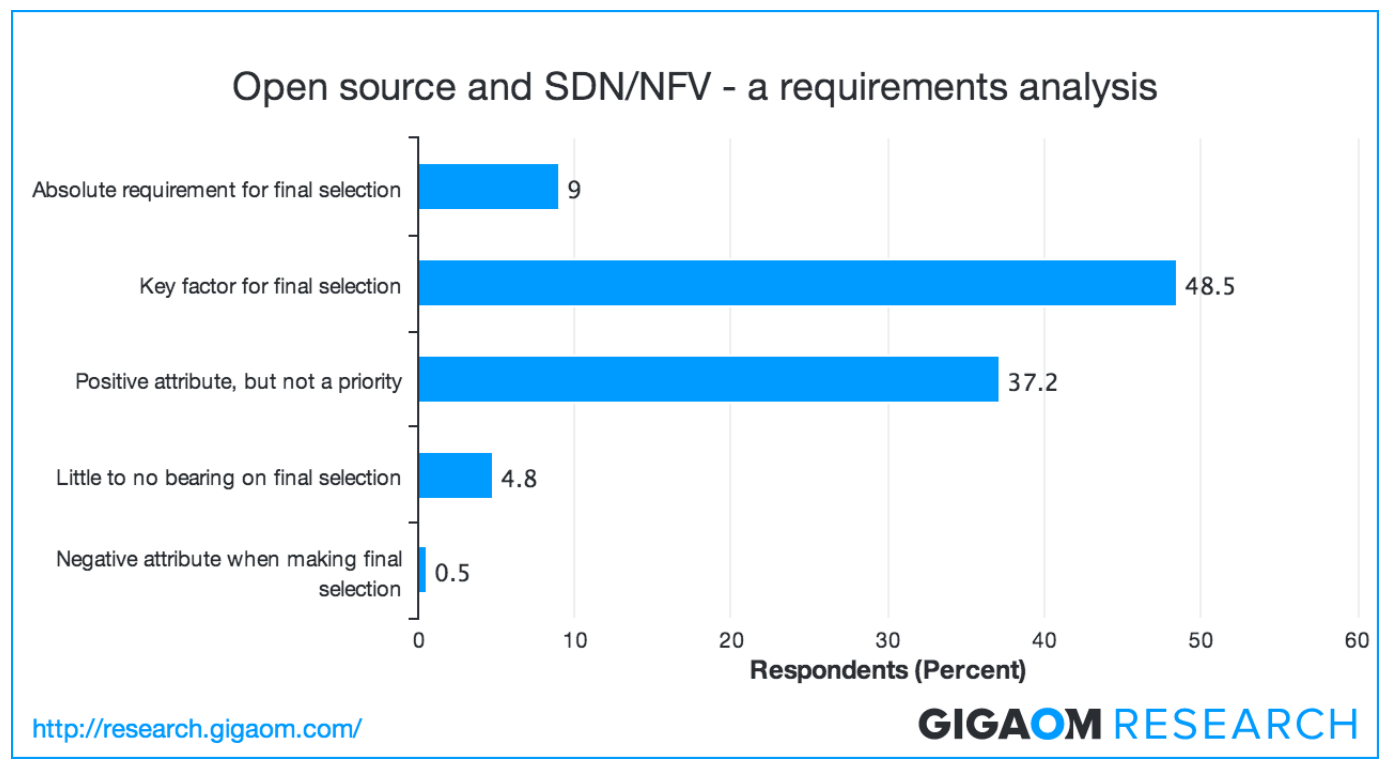
\includegraphics[width=10cm]{open-source-requirement-operator-view-00.png}
  \end{figure}
\end{center}

\end{frame}

\section{License}

\begin{frame}[allowframebreaks]
\frametitle{Licsense}

\begin{itemize}
 \item EPLv1.0:\linebreak
 - Open Source License, recognized by OSI and FSF\linebreak
 - GPL imcompatible\linebreak
 - Weak Copyleft License: Distribution of object code can be done under other license agreement\linebreak
 - Reasons from OpenDaylight to use EPLv1.0:
 \begin{itemize}
   \item FLOSS
   \item Java-based project
   \item 3rd party libraries compatiblity (Maven, OpenVSwitch, OpenFlow Java)
   \item Avoid licensing fragmentation
 \end{itemize}
\end{itemize}

\end{frame}

\section{Bylaws}

\begin{frame}[allowframebreaks]
\frametitle{Bylaws}

\begin{itemize}
  \item Name, Purposes, Oficces
  \item Members, Actions of Members
  \item Directors, Committees, Officers
  \item Notices, Indemnification
  \item Books and Records
  \item Transactions, Grants, Contracts and Loans
  \item General provisions
  \item Antitrust, Competition and Availability of Intellectual Property
  \item Ammendments
\end{itemize}

\end{frame}

\end{document}
